\section{Experimental Setup}
\label{sec:experimentalsetup}

\subsection{Dataset and Point-in-Time Data Contract}
The daily universe spans information technology (FPT, CMG), banking (VCB, MBB), retail (MWG), food/beverages (VNM, BHN) and aviation/tourism (HVN, VJC). This is a purposive, non-representative sample: BHN, CMG, FPT, HVN, MBB, MWG, VCB, VJC and VNM. The reconstructed vnstock/VCI price snapshot covers observed vendor sessions from 2020 through September 2026. It is not an authenticated submission-time snapshot. Contradictory BHN OHLC data trigger the frozen valid-suffix policy; insufficient subsequent warm-up excludes BHN from three early blocks. No price is corrected to improve a result. This leaves 102 eligible cells of the 12-date by nine-symbol grid in Figure~\ref{fig:calendar}.

\subsection{Walk-Forward Protocol}
Six blocks cover 2023 H2, 2024 H2, 2025 H1, 2025 Q4, 2026 Q2 and 2026 Q3, with two scheduled dates per block. These are twelve selected dates, not a continuous multi-year daily backtest. Cross-symbol observations share calendar shocks. The 51 eligible symbol--block scopes contain chronological train/validation/test partitions: every train label exits before validation starts, and every validation label exits before the first test decision. Cutoffs require the frozen history length; label spans touching the next partition are purged.

The reduced scope was amended after some inference to complete a bounded historical study. Its 375 registered Decisions include 193 explicitly reused successful executions and 182 further successes. The factorial subset was selected by metadata (symbol/date round-robin), not prediction quality, but this does not make the overall amendment preregistered. The larger legacy grids remain incomplete/superseded. Table~\ref{tab:scope} distinguishes shared r0 calls, additional realizations and the separate factorial panel; their observations are not summed as independent markets.

\begin{figure}[htbp]
\centering
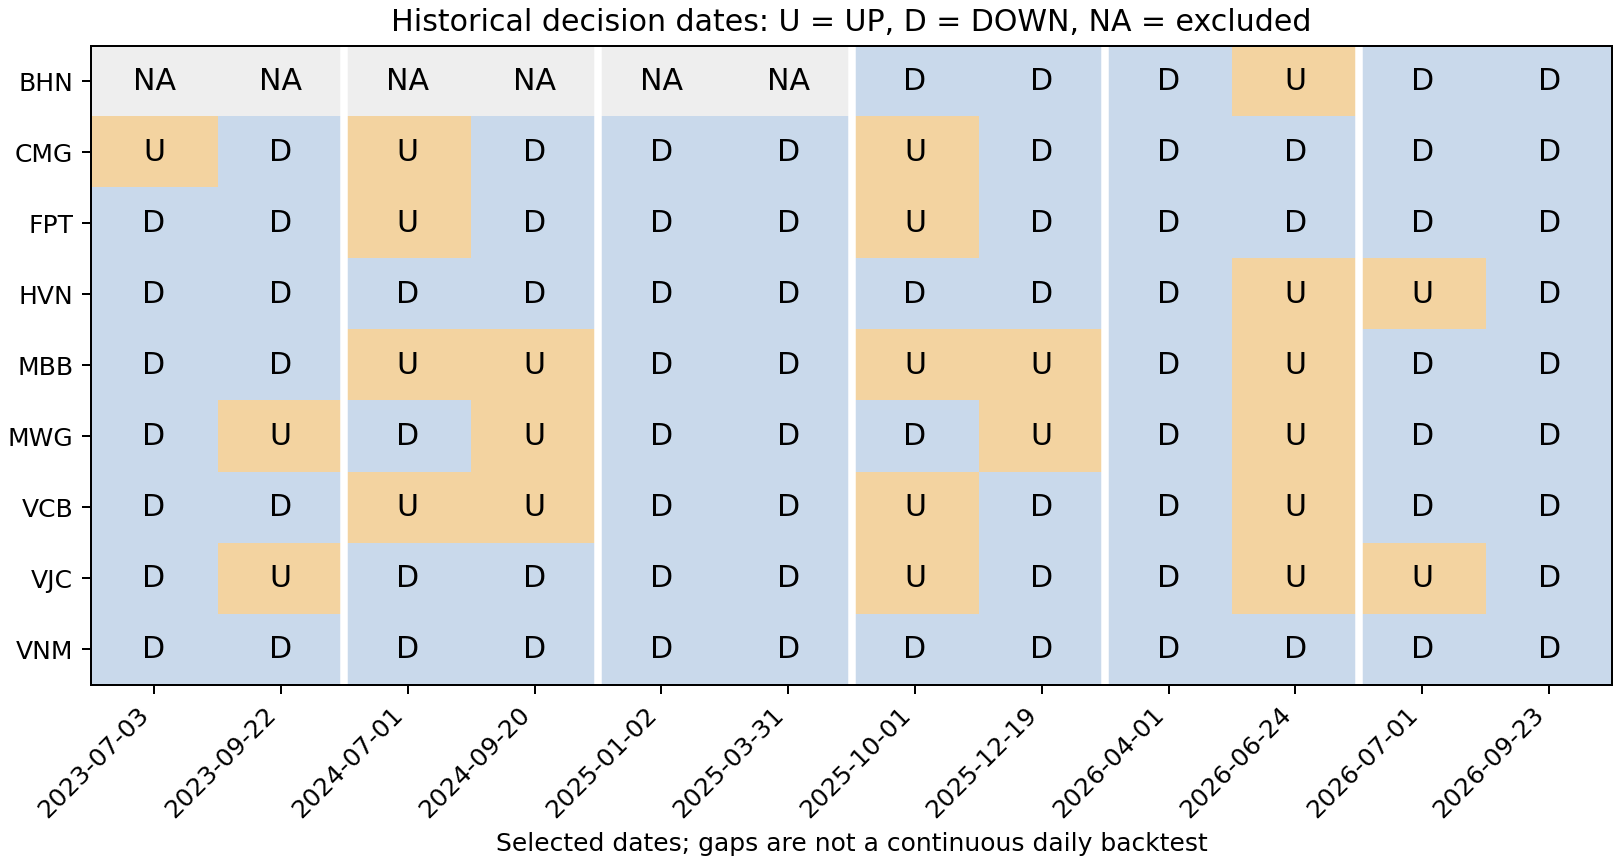
\includegraphics[width=\textwidth]{figs/final_calendar.png}
\caption{Selected historical decision dates and eligibility across nine equities. Missing BHN cells remain excluded rather than being filled with CASH predictions. Labels are shared evaluation truth, not a visualization selected from Full's successful forecasts.}
\label{fig:calendar}
\end{figure}
\begin{table}[p]
\centering\small
\setlength{\tabcolsep}{3pt}
\renewcommand{\arraystretch}{1.15}
\caption{Evaluation scopes and prompt variants in the frozen historical study. Shared main/upstream executions are counted once.}
\label{tab:scope}
\textbf{A. Recorded supports}\par\smallskip
\begin{tabular}{lrrrrrrr}
\hline
Scope & $N$/exec. & Symbols & Dates & Blocks & UP/DOWN & Exec. & Decisions \\
\hline
Main & 102 & 9 & 12 & 6 & 25/77 & 1 & 204 \\
Upstream & 9 & 9 & 3 & 3 & 2/7 & 3 & 54 \\
Factorial & 9 & 8 & 4 & 3 & 2/7 & 3 & 135 \\
\hline
\end{tabular}\par\medskip
\textbf{B. Prompt sections}\par\smallskip
\begin{tabular}{llll}
\hline
Variant & Factors & Sentiment & Representation \\
\hline
B & -- & -- & Shared price reports \\
A & Current & -- & Five-row factorial \\
S & -- & Current & Factorial \\
AS & Current & Current & Compact main / five-row factorial \\
P & Past donor & Current & Five-row factorial \\
\hline
\end{tabular}\par\medskip
\begin{minipage}{\textwidth}\footnotesize Main uses B/AS; upstream uses B/AS; factorial uses B/A/S/AS/P. Class counts are per execution. Upstream includes 18 main r0 calls: 204+54+135-18=375 unique Decisions. P preserves current names/schema/missingness and sentiment, replacing factor values/signals/skill metadata by one past train-only rank-vector donor.\end{minipage}
\end{table}


\begin{figure}[!htbp]
\centering\begin{tikzpicture}[x=1cm,y=1cm,>=Latex,
 box/.style={draw=blue!55!black,fill=blue!4,rounded corners,align=center,text width=4.1cm,minimum height=1.5cm,font=\footnotesize},arr/.style={->,thick}]
\draw[->,thick] (-0.3,0)--(14.5,0);
\node[font=\footnotesize] at (7.1,-0.9) {Observed bar position};
\draw[very thick,blue!60!black] (0,0.2)--(8.4,0.2);
\node[above,align=center,font=\small] at (4.2,0.3) {Chart window $[e-45,e)$\\Only bars through decision $d=e-1$ are visible};
\foreach \x/\lab in {0/{e-45},8.4/{d=e-1},10/{e},13.6/{e+2}}{\draw (\x,-0.12)--(\x,0.12);\node[below,font=\small] at (\x,-0.15) {$\lab$};}
\draw[<->,thick,orange!80!black] (10,1.5)--(13.6,1.5);
\node[above,align=center,font=\small] at (11.8,1.6) {Entry Open to exit Close\\$L=3$ observed bars};
\node[box] (t) at (2,-2.5) {Chronological training\\Labels mature before validation};
\node[box] (v) at (7.1,-2.5) {Validation / purge\\Labels exit before first test decision};
\node[box] (q) at (12.2,-2.5) {Frozen test dates\\Two dates per block; six blocks};
\draw[arr] (t)--(v);\draw[arr] (v)--(q);
\node[align=center,text width=14.0cm,font=\footnotesize] at (7.1,-4.5) {Shared reports $\rightarrow$ variant Decisions $\rightarrow$ immutable truth and separate accounts.\\Twelve dates / 102 eligible units; no synthetic bars and no uniform $S=3$ grid.};
\end{tikzpicture}

\caption{Walk-forward time-index and split contract. The 45-bar chart ends at $d=e-1$, entry is at $e$ and the $L=3$ target is at $e+2$. The final study visits twelve selected dates across six blocks; it does not use a uniform $S=3$, twenty-point grid. Outer cutoff isolation does not certify native row-wise causality.}
\label{fig:walkforward}
\end{figure}

\subsection{Paired Baseline and Disentangled Ablations}
All nine classifiers use the same 102 main units and net target. CASH and always-LONG are constant predictions; always-LONG closes and pays costs every cycle. Train-majority uses purged training labels, choosing CASH on a tie. Momentum predicts LONG for a strictly positive trailing 20-session return. Logistic-price uses numerical price features; logistic-matched adds the recorded factor/sentiment/missingness inputs. Imputation, scaling, regularization and decision threshold selection follow chronological train/validation rules; final logistic refits use matured train plus validation only. We reuse their saved predictions rather than refitting after observing outcomes. The fixed factor-vote comparator uses training-fitted medians/orientation and differs from the native top-five policy and the auxiliary numeric-control study.

Matched numerical inputs do not equal chart images, report wording or pretrained knowledge. Full--Base differences likewise include prompt structure, report length and propensity to choose CASH. The upstream panel has nine units, B/AS and three regenerated upstream realizations with a Decision execution per realization. The factorial panel has nine different-support units, B/A/S/AS/P and three Decision executions with fixed upstream. Both have two UP/seven DOWN per execution, but only the former covers nine symbols. We do not infer main-grid variability or separate upstream/Decision variance components from their SDs.

P retains current factor names, headings, schema/missingness and sentiment, replacing scalar values, signals and skill fields using a predetermined earlier train-only rank-vector donor. Donor label exits precede validation/test. Rank mapping is not name-matched covariance preservation, a placebo distribution or exposure matching. Five explicit rows reach each A/AS/P factorial prompt. Main/upstream compact prompts are a separate representation family. Interaction is defined as $AS-A-S+B$; the observed best-single gap $AS-\max(A,S)$ is a different, post-hoc diagnostic and not an eighth factorial contrast.

\subsection{Account and Statistical Metrics}
BA averages UP and DOWN recall; MCC and both-class precision/recall accompany ordinary accuracy and LONG rate. Pooled metrics retain actual class supports. Symbol macro means are unweighted and report planned/defined denominators. Missing class support or a degenerate MCC denominator yields NA, not zero. Main contrasts use 10,000 paired whole-block resamples, seed 20261102, retaining dates, cross-section, variants and eligibility together. Repeat diagnostics jointly resample recorded blocks and paired execution indices. Intervals condition on finite draws; undefined counts remain visible. Circular block lengths, leave-one-block-out and Bartlett HAC at lags 0/1/2 are sensitivity diagnostics. HAC uses calendar-aligned accuracy differences in fixed-universe panels, with a $t(n_{dates}-1)$ reference; few clusters, irregular gaps and post-inference additions prevent calibrated significance or power claims.

To specify the classification estimand, let TP/FN count UP outcomes and TN/FP count DOWN outcomes. We use
\begin{equation}
 \begin{aligned}
 BA&=\frac12\left(\frac{TP}{TP+FN}+\frac{TN}{TN+FP}\right),\\
 MCC&=\frac{TP\,TN-FP\,FN}{\sqrt{(TP+FP)(TP+FN)(TN+FP)(TN+FN)}}.
 \end{aligned}
 \label{eq:classification_metrics}
\end{equation}
The relevant metric is undefined when a required denominator is zero. Macro means average defined symbol-level values while retaining the planned and defined denominators. A CASH rule can have high ordinary accuracy in a DOWN-heavy sample without discriminating the two classes.

Each of 51 symbol--block accounts starts with VND50 million, without cross-symbol capital competition. LONG follows Eq.~\ref{eq:netlabel}; CASH stays flat. Continuous hold buys once from the first entry through the last scheduled exit, including gaps, and is not a tenth classifier. Wealth includes pending receivables and residual shares at recorded mark-to-market prices. Daily-close drawdown uses an initial-capital anchor. Where supplied in companions, daily Sharpe uses population SD and a 252-session convention with zero risk-free rate; the retained Sortino convention uses SD of negative daily observations, not downside RMS. Annualised cycle ratios are NA for the irregular/gapped main schedules, and are not presented as investment-quality estimates from a handful of trades.

The reference assumes fractional fills at recorded prices and two-leg fees/slippage. Shares are assumed sellable in the afternoon of T+2 conditional on allocation and fill; sale proceeds are pending until the specified settlement phase. This convention follows the archived settlement source \cite{vsd2022settlement}. L=3 is a fixed observed-bar protocol choice, not an optimized horizon. Daily OHLC cannot authenticate opening-auction queues, price-limit fills, partial fills or correct volume units. All twelve sensitivities, including pending cash, advances, cost changes, sell charge, no-fill/delay proxies and lot/capacity assumptions, remain in \ref{app:additional}. Venue/calendar review flags, including ten HVN unit flags, are retained rather than converted to certified fills or synthetic CASH.

\subsection{Implementation and Robustness Design}
Archived SDK aliases are \texttt{openai/gpt-oss-20b} for text and \texttt{qwen/qwen3.8-27b} for vision. Configured temperature zero appears as $10^{-8}$ in observed SDK metadata; no hosted decoding seed is recorded. Text/vision output caps are 2,048/1,024 tokens. Retry/checkpoint records preserve individual attempts and completed outputs. Aliases and 40 response fingerprints do not authenticate an immutable weight revision or historical provider catalogue; 91 original Pattern requests lack epoch/provider-org fields and remain unknown. Offline replay reproduces saved-prediction metrics, not a fresh hosted inference experiment.

The closure contains 649 attempts, 615 successes and 34 errors, including 120 original Pattern calls replayed as shared dependencies. Observed usage totals 1,063,328 prompt and 340,736 completion tokens. Error usage/latency and monetary billing are unknown. Pattern tokens/latency describe original calls, not replay lookup cost; successful callback elapsed times are not wall-clock runtime. Full accounting, pins and hashes are in repository artifacts rather than an implementation appendix.
